\documentclass[class=book,crop=false]{standalone}
\usepackage{../style}
\begin{document}
\chapter{Arrays}
An array is a group of variables or constants, all of the same type, which are referred to by a single name. The values in the group occupy consecutive locations in the computer memory. An individual value within the array is called an array element; it is identified by tge name of the array together with a subscript pointing to the particular location within the array.
\begin{figure}[H]
    \centering
    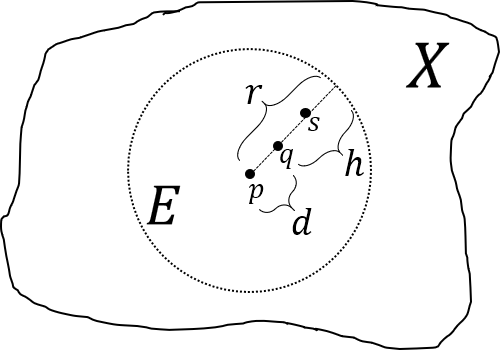
\includegraphics[scale=.75]{Picture1.png}
    \caption{The elements of an array occupy successive locations in a computer memory}
    \label{fig:array}
\end{figure}
For example, the first variable shown in figure \ref{fig:array} is referred as a(1). The subscript of an array is of type \code{integer}. Either constants or variables may be used for array subscripts. Arrays can be extremely powerful tools for manipulating data in Fortran. They permit us to apply the same algorithm over and over again to many different data items with simple \code{do} loops. It is possible to manipulate and perform calculations with individual elements of arrays one by one, with whole arrays at once, or with various subsets of arrays.\\

Mathematically, we often denote the whole array by its subscripted name. e.g., x for $ \{x_i\} $ or a for $ \{a_{ij}\} $. Whist subscripted variables are important in any programming languages, it is the ability to refer to ah array as a whole, without subscripts, which makes Fortran particularly valuable in engineering. The ability to refer to just segments of it, e.g., the array section x(4:10) is just like the icing on the cake.
\section{Some Terminology of Array}
\subsection{\code{Rank}}
The number of subscripts declared for a given array is called the \code{rank} of the array.
\subsection{\code{Dimension}}
The \code{dimension} attribute in the type declaration statement declares the size of the array .
\subsection{\code{Size}}
The \code{size} of an array is the total number of element declared in that array.
\subsection{\code{Extent}}
The number of elements in a given dimension of an array is called the \code{extent} of the array in that dimension.
\subsection{Shape}
The shape of an array is defined ad the combination of its \code{rank} and the \code{extent} of the array in each \code{dimension}. Thus two arrays have same shape if they have the same \code{rank} and the same \code{extent} in each \code{dimension}.
\section{Array Declaration}
Like any other variable arrays need to be declared at the start of a program unit and memory space assigned to them.

However, unlike scalar variables, array declarations requrire both a type (\code{integer, real, complex, character, logical} or derived type) and a \code{size} or \code{dimension} (number of elements). For e.g.,
\begin{lstlisting}[numbers=none,escapechar=\%]
    real x(100), y(100)
    %or using dimension attribute%
    real, dimension(100) :: x, y
\end{lstlisting}
We might need to change array size consistently in many places, it is safer practice to declare array size as a single parameter. e.g.,
\begin{lstlisting}[numbers=none]
    integer, parameter :: maxsize = 100
    real x(maxsize), y(maxsize)
\end{lstlisting}
By default, the first element of an array has subscript 1. It is possible to make the array start from subscript zero (or any other positive or negative integer) by declaring the lower bound as well. For example, to start at zero instead of one,
\begin{lstlisting}[numbers=none]
    real x(0:99)
\end{lstlisting}
\section{Dynamic Arrays}
An obvious problem arises, what if the number of points n is greater that the declared size of the array (here, 100)?

One not-very-satisfactory solution is to check for adequate space, prompting the user to recompile if necessary with a larger array size.
\begin{lstlisting}[numbers=none]
    read (10,*) n
    if (n > maxsize) then
        print*, "Sorry, n>maxsize. Please recompile with larger array"
        stop
    end if
\end{lstlisting}
A far better solution is to use dynamic memory allocation; that is, the array size is determined (and computer memory allocated) at run-time, not in advance during compilation. To do this one must use \code{allocatable} arrays as follows\begin{enumerate}
    \item In the array declaration statement, use the \code{allocatable} attribute, e.g.,
    \item \begin{lstlisting}[numbers=none]
        real, allocatable :: x(:), y(:)
    \end{lstlisting}
    Note that the shape, but not size is indicated at compile time by a single colon (:).
    \item Once the size of the array has been identified at run-time, allocate them the required amount of memory:
    \begin{lstlisting}[numbers=none]
        read (10,*) n
        allocate (x(n), y(n))
    \end{lstlisting}
    \item When the arrays are no longer needed recover memory by deallocating them:
    \begin{lstlisting}[numbers=none]
        deallocate (x, y)
    \end{lstlisting}
\end{enumerate}
\section{Elemental Operations}
Some times we want to do something to every element of an array.\\The expression \code{x * x} is a new array with elements $ \{{x_i}^2\} $.\\
The expression \code{sum (x * x)} therefore produces $ \sum {x_i}^2 $\\
Using many of these features a shorter version of the above program is given bellow
\lstinputlisting{regressionElemental.f90}
\section{Matrices and Higher-Dimension Arrays}
A m$ \times $n arrays of number of the form $ \begin{pmatrix}
        a_11 &\dots & a_1n\\
        \vdots & \ddots & \vdots\\
        a_m1 & \dots & a_mn
    \end{pmatrix} $ is called a matrix (or rank-2 array). The typical element if denoted by $ a_ij $. It has two subscripts. Fortran allows matrices and infact, arrays of upto 7 dimension. In Fortran, the declaration and use of a real $ 3\times 3 $ matrix might look like\begin{lstlisting}[numbers=none]
        real A(3,3)
        A(1,1) = 1.0; A(1,2) = 2.0
        A(1,3) = 3.0; A(2,1) = 4.0    etc
    \end{lstlisting}
\section{Matrix Multiplication} Suppose A, B and C are $ 3\times3 $ matrices declared by\begin{lstlisting}[numbers=none]
    real dimension (3,3) :: A, B, C
\end{lstlisting} 
The statement \code{C=A*B} does element-by-element multiplication; each element C is the product of the corresponding elements in A and B.

To do "proper" matrix multiplication use the standard \code{matmul} function: \begin{lstlisting}[numbers=none]
    C = matmul(A, B)
\end{lstlisting}
A similarly use =ful function is that computing the transpose of a matrix :
\begin{lstlisting}[numbers=none]
    C = transpose (A)
\end{lstlisting}
\section{Array Constants} Array constants may also be defined. An array constant is an array consisting entirely of constants. It is defined by placing the constant values between special delimiters, called array constructors. The starting delimiter of a Fortran array constructor is \code{(/} (old) or \code{[} (modern) and the ending delimiter of an array constructor is \code{/)} or \code{]}. e.g., \code{(/ 1, 2, 3, 4 /)} or \code{[ 1, 2, 3, 4 ]}
\end{document}